\documentclass{article}

\usepackage[brazil]{babel}
\usepackage{graphicx}
\usepackage{hyperref}
\usepackage{geometry}
\geometry{a4paper, margin=2cm}
\usepackage{siunitx}
\usepackage{subcaption}

\setlength{\parindent}{0pt}
\setlength{\parskip}{0.5em}

\title{Acústica da Marimba}
\author{Gabriel Haruo Hanai Takeuchi (NUSP: 13671636)}
\date{}

\begin{document}

\maketitle

\section{Introdução}

A marimba é um instrumento de \textbf{percussão} da classe dos \textbf{idiofones} de \textbf{uma dimensão}. É composta por \textbf{barras}, que podem ser percutidas por \textbf{baquetas}, e \textbf{ressoadores}, que potencializam a intensidade do som.

\begin{figure}[h!]
  \centering
  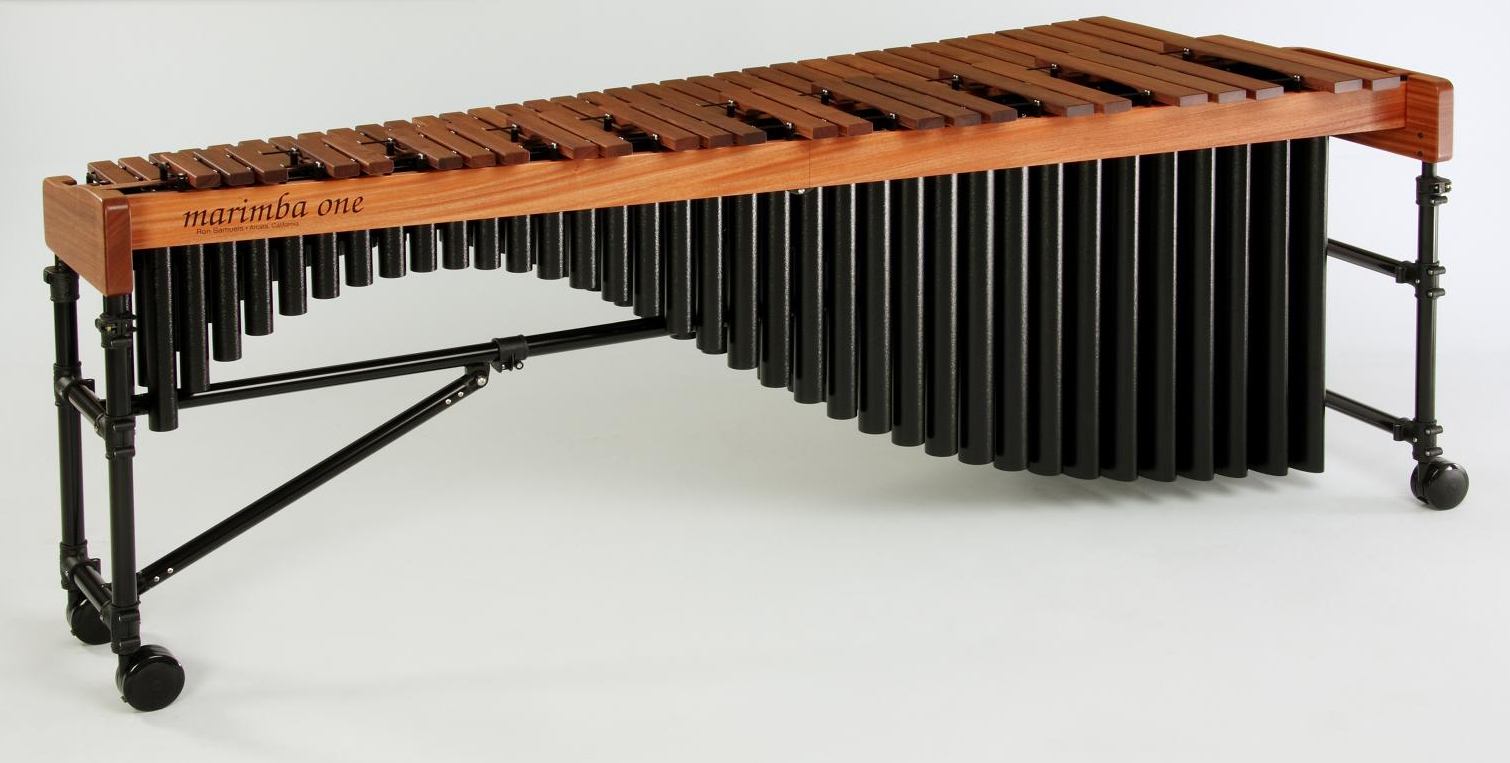
\includegraphics[width=0.8\textwidth]{Marimba_One_4000_Series.jpg}
  \caption{Marimba One 4000 Series~\cite{wiki:marimba}}
  \noindent 
\end{figure}

\section{Estrutura}

\subsection{Barras}

As barras (ou lâminas) da marimba são feitas de madeira de pau-rosa ou fibra de vidro, com largura variando de \SI{4.5}{\centi\meter} a \SI{7.5}{\centi\meter}. A espessura de uma barra é composta por extremidades mais grossas e uma região central mais fina (um arco escavado), o que permite uma afinação precisa controlando a massa do objeto.

\begin{figure}[h!]
	\centering
	\begin{subfigure}{0.45\textwidth}
		\centering
		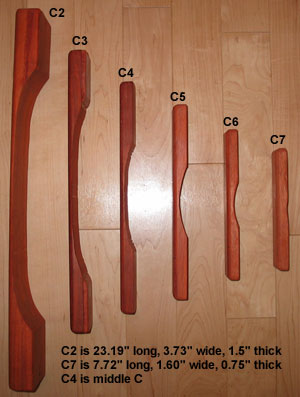
\includegraphics[height=245px]{marimba_bars.jpg}
	\end{subfigure}
	\hfill
	\begin{subfigure}{0.45\textwidth}
		\centering
		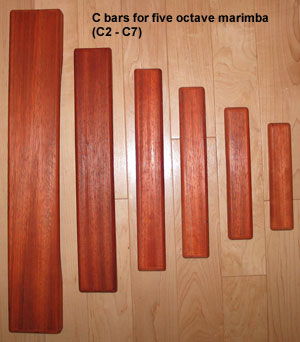
\includegraphics[height=245px]{marimba_bars-top.jpg}
	\end{subfigure}
	\caption{Vista lateral e superior das barras da marimba~\cite{lafavre_tuning_marimba}}
\end{figure}

O movimento vibratório das barras é tratado como unidimensional, ou seja, as vibrações ocorrem ao longo do comprimento da barra.

São suspensas por meio de uma corda de algodão com tensão regulável. A escolha do algodão é dada pela sua flexibilidade, o que evita que a corda não vibre por ressonância externa e introduza qualquer ruído indesejado. A importância da tensão ser regulável é destinada ao

\begin{itemize}
  \item Controle de vibração: uma corda muito tensa pode restringir a vibração das barras, enquanto uma muito frouxa pode não dar estabilidade o suficiente para as barras vibrarem adequadamente;
  \item Controle de altura das barras: a tensão adequada garante que uma sequência de barras, aos quais possuem tamanhos e massas variadas, estejam alinhadas.
\end{itemize}

As barras são percutidas por baquetas adequadas ao instrumento, e são excitadas no ponto médio da barra para maximizar a amplitude da vibração.

\subsection{Ressoadores}

% O tubo é fechado em uma extremidade -> afeta o comprimento de onda
\begin{figure}[h!]
	\centering
	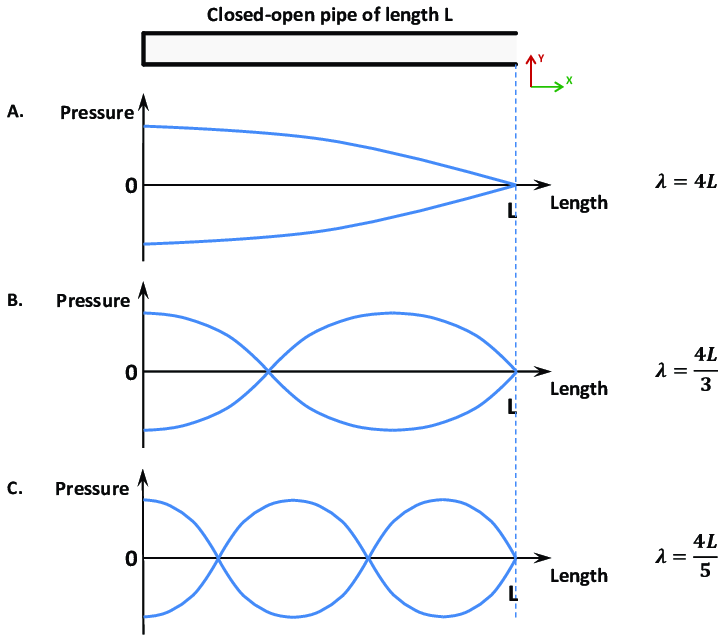
\includegraphics[width=0.6\textwidth]{Harmonics-of-a-closed-open-pipe-in-three-different-wavelengths-A-Four-times-the-length.png}
	\caption{Harmônicos de um tubo fechado-aberto em três comprimentos de onda diferentes: A. Quatro vezes o comprimento do tubo (4L) B. Quatro terços do comprimento do tubo (4L/3) e C. Quatro quintos do comprimento do tubo (4L/5)~\cite{closed_open_pipe}}
\end{figure}

% Enfatiza a fundamental, aumenta a intensidade sonora, mas diminui o tempo de decaimento


% E2 em 60dB sem ressoador -> 3.2s de decaimento; com ressoador -> 1.5s

\section{Sonoridade}

% Afinação dos modos 1,4,9-10

A tessitura da marimba está contida no intervalo de A2 (\SI{110}{\hertz}) até C7 (\SI{2093}{\hertz}), sendo que os graves podem ser estendidos até C2 (\SI{65}{\hertz}). 

As barras são afinadas para os modos 1, 4, 9 e 10.

\bibliographystyle{plain}
\bibliography{references}

\end{document}